\RequirePackage[T1]{fontenc}
\documentclass[journal]{IEEEtran}
\usepackage[UTF8,scheme=plain,fontset=none]{ctex}
\setmainfont{texgyretermes-regular.otf}[BoldFont=texgyretermes-bold.otf,
 ItalicFont=texgyretermes-italic.otf,BoldItalicFont=texgyretermes-bolditalic.otf]
\setCJKmainfont{FandolSong-Regular.otf}[BoldFont=FandolSong-Bold.otf,
 ItalicFont=FandolKai-Regular.otf,SmallCapsFont=FandolSong-Regular.otf,Script=Default]
\setCJKsansfont{FandolHei-Regular.otf}[BoldFont=FandolHei-Bold.otf,Script=Default]
\setCJKmonofont{FandolFang-Regular.otf}[Script=Default]
\usepackage{amsmath,amssymb,booktabs,cite,xurl,graphicx}
\usepackage[hidelinks]{hyperref}
\interdisplaylinepenalty=2500
\begin{document}
\title{已知总时长与同段信息共享下的分段运行时间估计}
\author{}
\maketitle
\begin{abstract}
公交运行分析需要定位耗时较长的站间区间，但稀疏观测往往只覆盖整趟行程及少量局部位置。已知运行总时长不能唯一确定各区间耗时，相同区间在不同行程中也存在差异。Ours结合重复区间共享估计与有界行程修正，再按已知总时长进行比例缩放。在公开Astana公交数据开发集上比较三种局部标签预算。在验证集选出的主比较中，Ours的MAE点估计在1\%和5\%预算下低于同输入直接预测，分别相差0.579秒和0.075秒；在10\%预算下则更高。九组配对运行中，Ours分别在8、6和0组取得较低误差。标签极少时，同段均值仍优于Ours。通过验证集选择0.5权重的Ours+Direct集成在三种预算下均低于直接预测，但它是独立的集成预测器，且1\%预算下仍不及同段均值。相同标签数量在不同区间覆盖布局下也产生不同误差。最终时间划分未参与评价，因此这些结果仅反映开发集比较。
\end{abstract}
\begin{IEEEkeywords}
分段运行时间估计，已知总时长，同段信息共享，稀疏监督，公交运行。
\end{IEEEkeywords}
\section{引言}
公交运营人员分析线路运行时，需要知道耗时发生在哪些站间区间。整趟行程的总时长可以用于比较线路效率，却不能说明某次延误主要发生在前段还是后段。分段运行时间能够支持瓶颈区间筛查和分时段运行比较。然而，完整局部记录依赖持续定位与可靠的站点匹配，设备采样间隔和记录缺失会使部分区间不可观测。利用已知总时长和有限局部观测估计各段时间，因而是旅行时间推断中的实际需求\cite{hellinga2008,hofleitner2011,yin2015entryexit}。

本文研究已经完成行程的分段运行时间估计。这里的分段是有向站间区间，总时长是各区间运行时间之和，不包含停站时间。它与起终点时间戳之差有所区别：后者还可能包含停站和其他非运行时间，需要先分离这些部分并对齐区间边界。实验对公开数据的运行时间求和构造已知总时长，以考察精确总时长条件下的分段估计。

考虑一趟经过三个连续区间、运行总时长为十分钟的行程。$(2,3,5)$和$(5,3,2)$分钟是两组可行分配。训练中即使提供中间区间三分钟的标签，也无法区分这两种分配；推理时不提供当前行程的局部标签。这两组结果分别将末段和首段识别为最耗时的位置，可能导致不同的运营判断。其他行程中相同区间的记录能够帮助区分这两种分配；但如果当前行程的出发时段或路线条件发生变化，直接沿用历史平均值又可能掩盖差异。这个例子说明，模型既需要利用同一区间的重复观测，也需要判断当前行程应如何偏离平均规律。

已有研究通过自由流信息、局部时间分布或统计交通流模型为总时长分解提供依据\cite{hellinga2008,hofleitner2011}。路径不完整时，路段推断还需联合估计经过的路径与局部时间\cite{yin2015entryexit,sun2022prltte}。本文关注路径顺序已知、区间重复出现且部分单区间标签可见的条件。这里不需要重新恢复路径，关键在于如何把跨行程可共享的信息与当前行程的差异结合起来，并保证分段输出符合已知总时长。

同段均值利用重复观测，却把随出发时段和行程条件变化的耗时视为固定值；本文的直接预测基线也共享区间嵌入并使用当前行程上下文，但直接输出正值分数，不设置单独的重新分配分支。本文将两者分开建模：共享分支根据上下文估计基础时间，序列分支提出有界调整，随后按已知总时长比例缩放。本文的贡献是这一分配参数化及其在稀疏标签下的分析；其精度能否优于直接预测仍需由实验检验。

实验结果进一步限定了这一设计的作用。标签极少时，同段均值仍是有竞争力的基线；在较高标签预算下，本文方法改善了同段均值的误差，但对同输入直接预测没有稳定优势。关闭行程修正会使同一模型的误差上升，说明修正分支有助于基础估计，却不能据此推断完整方法优于直接预测。相同标签数量若只覆盖较少区间身份，误差会显著增加；在身份集合和逐身份标签数相同的控制中随机改变标签位置，也没有恢复较广覆盖时的精度。由此可见，已知总时长排除了不满足总量的分配，却不能单独判定哪一种局部时间分配正确；方法能否作出有用判断，还取决于共享区间信息的覆盖程度。

\section{相关工作}
\subsection{已观测旅行时间的分解}
稀疏探测车辆的两次位置观测可能跨越多个道路链路，因此需要沿已识别路径分配两次观测之间的耗时。Hellinga等利用链路几何与自由流速度，将旅行时间分为自由流、拥堵和停止时间\cite{hellinga2008}。其拥堵似然利用前一采样区间的信息，停止似然则反映车辆位置与链路下游端的关系，最终通过对可能的拥堵程度积分得到时间分配。Hofleitner和Bayen从干道排队与驾驶行为的统计模型推导链路时间分布\cite{hofleitner2011}。这些分布由对数凹分量混合而成，整体分配问题并非凸问题；固定延迟模式后可得到凸子问题，进而采用枚举或基于EM的算法求解。两项研究均要求分配时间之和等于观测总时长。

网络层面的推断还可以结合多次行程的共同观测。Yin等从行程进出记录推断链路时间分布，研究高斯似然、路径未知时的混合模型估计，以及面向更一般分布的行程拆分\cite{yin2015entryexit}。PR-LTTE交替利用行程距离与耗时恢复路径，并通过非负最小二乘估计链路时间\cite{sun2022prltte}。这些方法估计共享的道路链路量，部分方法还需恢复缺失路径。本文已知有序的有向公交站间区间，每个区间可以跨越多个道路链路；共享估计随可观测上下文变化，重新分配则随具体行程变化。NNLS-Ridge参照用于检验这一已知序列条件下的固定区间身份系数。

\subsection{旅行时间表示学习}
DeepTTE结合地理卷积与循环网络，同时学习整条路径和局部路径的旅行时间\cite{wang2018deeptte}。其局部标签来自GPS窗口的时间戳差，窗口之间可以重叠；整条路径时间由独立的注意力预测头输出。DutyTTE针对未提供路线时的旅行时间不确定性，将预测路径对齐与上下文相关的区间不确定性建模结合起来\cite{mao2025dutytte}。这类设计利用局部观测与路线表示预测尚未知晓的行程耗时。

ProbETA与重复链路的信息共享更为接近\cite{xu2025probeta}。Xu等将链路时间写为共享均值、日期随机效应和行程随机效应之和，通过学习低秩协方差表示描述行程之间和行程内部的依赖。训练利用行程总时间与时间戳生成的子行程时间构建联合似然，推断则结合邻近已完成行程，对查询行程的时间分布作条件估计。这是一种以概率模型组织共享链路证据的方式。本文已知查询行程的总时长，由有限单区间标签监督内部时间分配；行程修正的幅度相对于共享基础时间受到限制，并在本次行程内加和为零，其作用是调整分配比例。

\subsection{聚合监督与加和一致性}
聚合观测学习研究如何根据组级监督估计个体标签。Zhang等推导聚合观测的似然，并在条件独立假设下讨论由均值或总和监督进行回归\cite{zhang2020aggregate}。其中，聚合误差用于训练个体预测器。本文通过比例缩放使每次输出严格符合给定总量，因此最终输出的总和误差不提供学习信号。训练和模型选择分别使用训练集与验证集中的可见单区间标签。

预测协调从另一个角度处理加和一致性。MinT利用预测误差协方差结合不同聚合层级的预测，使协调后的预测满足加和关系\cite{wickramasuriya2019mint}。本文的总量是已观测输入，需要学习的是未知的区间份额，随后将其缩放到该总量。相应地，实验在相同输入、标签预算和最终缩放下比较“共享基础估计加行程修正”与直接区间预测，检验施加一致性约束后如何学习行程内部的时间分配。

\section{方法}
\subsection{任务定义}
训练输入为有向站间区间序列、上下文特征及行程运行总时长，监督只使用可见的单区间标签。推理使用相同类型的输入，估计当前行程各区间的运行时间。本文的区间连接两个相邻站点，可能跨越多条道路边。重复区间通过共享参数利用其他行程的观测，同时保留不同出现之间的耗时差异。

行程$q$包含$L_q$个有序区间，第$i$个区间的身份、特征和运行时间分别为$s_{qi}$、$x_{qi}$和$t_{qi}\geq0$，已知运行总时长为$T_q>0$。将有序特征和身份记为$X_q$，模型输出满足
\begin{equation}
\hat{\boldsymbol t}_q=f_\theta(X_q,T_q),\qquad
\hat{\boldsymbol t}_q\geq0,\quad
\boldsymbol1^\top\hat{\boldsymbol t}_q=T_q.
\label{eq:task}
\end{equation}
总时长与区间目标采用相同的时间定义和观测边界，当前行程的局部真值不作为推理输入。

训练时仅集合$V$中的单区间标签可见。若一趟行程有$m<L_q-1$个不同位置的标签，加上总时长方程后，在严格正值的可行解附近仍有$L_q-m-1$个自由方向。在两个未观测区间之间转移少量时间，就能保持现有观测不变。这正是引言中首尾分配难以区分的原因，也是利用同段观测和上下文学习分配规律的依据。

\subsection{总体设计}
图\ref{fig:framework}展示三个步骤：根据区间身份和上下文估计基础时间，读取有序行程调整各段的相对分配，再将预测分配归一到已知总时长。两个分支通过最终分段输出接受局部监督；总时长不作为编码特征。同段信息由训练中共享的参数积累，无需在推理时额外输入历史时间标签。
\begin{figure*}[t]
\centering
\rule{0pt}{1.5in}
\caption{Ours总体结构。共享分支估计正值基础时间，序列分支生成有界零和修正，已知行程总时长由比例缩放施加。}\label{fig:framework}
\end{figure*}
\subsection{共享表示与序列表示}
模型为每个有效分量构造两类表示。共享表示$h^B_{qi}$由公共特征映射与身份嵌入组成，使相同身份的不同出现能够复用参数。序列表示$h^R_{qi}$在局部特征、身份与位置嵌入的基础上，加入有向邻接转移，再由Transformer处理有序序列。有效位置表示的均值经线性映射后回加到各位置，并进行层归一化。所有阶段均屏蔽填充位置。

两个标量网络分别生成基础值与修正分数。令$I_q$为有效位置集合。省略序列下标，有
\begin{align}
b_i&=\exp\bigl(\operatorname{clip}(g_B(h^B_i),-8,12)\bigr),\\
u_i&=g_R(h^R_i),\qquad
z_i=u_i-\frac1{|I_q|}\sum_{j\in I_q}u_j,\qquad i\in I_q.
\label{eq:heads}
\end{align}
截断避免指数运算溢出，$z_i$通过有效位置均值中心化。下一步再按基础比例中心化局部调整，以保证修正之和为零。由于共享特征包含日历等上下文，$b_i$随条件变化，不是固定历史均值。

\subsection{有界重新分配}
令$B=\sum_jb_j$、$p_i=b_i/B$，并取固定$0<\rho<1/2$，定义
\begin{align}
a_i&=\rho b_i\tanh(z_i),\\
\delta_i&=a_i-p_i\sum_j a_j,\qquad r_i=b_i+\delta_i.
\label{eq:redistribution}
\end{align}
第一项提出上下文相关的局部变化，第二项按基础比例去除其中的总量变化。由于$\sum_ip_i=1$，可得$\sum_i\delta_i=0$，从而$\sum_ir_i=B$。同时，
\begin{equation}
|\delta_i|\leq\rho b_i+p_i\rho B=2\rho b_i,
\end{equation}
因此
\begin{equation}
(1-2\rho)b_i\leq r_i\leq(1+2\rho)b_i.
\label{eq:positive}
\end{equation}
有效位置的修正后取值始终为正。主比较根据可见验证标签为每个预算分别选择$\rho$；固定$\rho=0.45$的控制实验单独报告。将修正分数置零时，$\delta_i=0$，只保留基础项。

幅度上界使行程调整保留与基础估计的联系，并直接保证正值；若基础估计偏差很大，这一上界也可能限制纠正能力。零和修正则去除行程分支的整体增减，使其专门处理各段之间的重新分配。最终缩放可以对任意正值向量保证加和一致，因此零和条件的作用是约束修正分支，而不是增加一个必要的守恒步骤。实验分别比较修正幅度及两种中心化形式，检验这些设计对误差的实际影响。

\subsection{已知总时长调整}
基础估计的加和不一定等于已知总时长。本文采用比例缩放满足式\eqref{eq:task}：
\begin{equation}
\hat t_i=T\frac{r_i}{\sum_jr_j}=T\frac{r_i}{B}.
\label{eq:rescaling}
\end{equation}
等价地，
\begin{equation}
\hat t_i=T p_i\left[1+\rho\left(\tanh z_i-\sum_jp_j\tanh z_j\right)\right].
\label{eq:shape}
\end{equation}
式\eqref{eq:shape}表明，基础估计与中心化修正决定行程内的比例，$T$决定整体尺度。有效位置保持非负，填充位置为零；浮点求和的舍入残差加到最大有效分量。固定$X$并改变总时长只会等比例改变输出。Ours与直接预测使用相同的最终调整，比较重点因而是局部分配，而非是否满足总时长。

\subsection{可见局部标签学习}
对于批次$\mathcal B$中的可见训练位置$V_{\mathcal B}$，最小化
\begin{equation}
\mathcal L_{\mathcal B}=\frac1{|V_{\mathcal B}|}
\sum_{(q,i)\in V_{\mathcal B}}h_\beta(\hat t_{qi}-t_{qi}),
\label{eq:loss}
\end{equation}
其中
\begin{equation}
h_\beta(e)=\begin{cases}
e^2/(2\beta),&|e|<\beta,\\
|e|-\beta/2,&\text{其他}.
\end{cases}
\end{equation}
实验取$\beta=5$秒。比例调整使同一行程的各段预测相互关联，可见位置的误差通过公共分母回传到两条分支。不可见标签不参与目标计算。缩放后的总时长误差恒为零，不能单独用于学习分配，因此主实验使用局部Huber损失，无标签参考采用均匀分配。重新分配与缩放的计算量为$O(L)$，宽度为$d$的自注意力计算量为$O(L^2d)$。

\subsection{完整标签下的可选辅助目标}
主实验只使用式\eqref{eq:loss}。报告的Singapore辅助运行禁用了历史侧路；在局部标签完整的条件下，另加入时长权重和前缀误差。若$M_{qk}=1$表示有效位置，前缀目标为
\begin{equation}
\mathcal L_P=\frac{\sum_{q,k}M_{qk}\left|\sum_{i\leq k}(\hat t_{qi}-t_{qi})\right|/\max(T_q,1)}{\sum_{q,k}M_{qk}}.
\label{eq:prefix}
\end{equation}
累计误差与归一化分母均只计有效区间，增加右侧填充不改变损失。辅助实验使用$\mathcal L_W+\lambda_P\mathcal L_P$，其中$\mathcal L_W$为按有效时长权重归一化的局部Huber损失。权重和训练配置见实验部分。额外历史标签条件下的同段对数时长目标在补充材料单独报告。

\section{实验}
主要比较采用Astana数据及相同局部损失和训练配置；Singapore辅助实验使用完整局部标签评价前缀目标。

\subsection{数据、时间定义与预处理}
Astana数据集\cite{astana2025}于2025年6月29日在Zenodo发布，采用CC BY 4.0许可，采集描述覆盖2024年7月至9月三条公交线路。使用的站间记录覆盖2024年7月29日至9月21日，共785,976条记录和19,769趟行程。预处理要求有向站点链连续、运行时间为5至1,800秒、停站时间为0至900秒；不满足条件的行程整趟删除。最终保留10,910趟、439,659个区间和586个有向区间身份。最长有效行程含55个区间，模型据此填充，未对更长行程截断。

区间身份由方向、起点和终点站标识构成，目标采用记录中的运行时间字段。各有效区间目标之和构成输入总时长，停站时间不计入目标。

行程按时间排序后以60\%/20\%/20\%划分。第一部分中5,891趟用于拟合、655趟用于选择检查点；中间20\%的2,182趟作为开发评价集。最后20\%未纳入本文报告（表\ref{tab:partitions}）。
\begin{table}[t]
\centering\footnotesize
\caption{Astana分区与有效标签规模。}\label{tab:partitions}
\begin{tabular}{lrr}\toprule
用途 & 行程数 & 有效区间数\\\midrule
模型拟合 & 5,891 & 237,203\\
检查点选择 & 655 & 26,561\\
开发评价 & 2,182 & 87,715\\
\bottomrule\end{tabular}
\end{table}

模型使用31项几何、路线、站点和出发日历特征，标准化参数仅由拟合数据估计。输入排除目标衍生统计、真实区间进入时间、标签质量字段及额外历史时间标签。

Singapore辅助数据覆盖2017年5月5日至6月19日。区间目标由相邻连续站点观测组的时间中点之差计算，未独立剥离停站时间。每个源记录取最长有效连续片段，要求至少8个区间、时长30至1,800秒、观测弦速度不超过25米/秒；最大长度87，不插值或跨记录拼接。训练日期为5月5日至6月5日，检查点选择为6月6日至8日，开发评价为6月10日至16日，中间留一天。分别使用50,000、5,000和10,000趟行程，开发评价含197,301个区间。该数据的目标定义与Astana不同，故结果分开报告。

\subsection{标签预算与训练设置}
训练与验证采用相同的标签比例，预算为1\%、5\%和10\%。训练分别开放2,372、11,860和23,720个标签，验证为265、1,328和2,656个。每个划分随机排列有效位置并按预算抽取，使用三组嵌套标签布局，每组进行三次独立初始化，因此每种神经方法在每个预算下有九次运行。两种方法共享配对初始化、批次和可见标签；不可见目标在训练及验证前屏蔽。

编码器宽度64，含两层Transformer和四个注意力头，前馈宽度256，dropout为零。主Ours/直接预测比较使用AdamW，初始学习率0.001并采用余弦退火，训练960步，每24步检查一次。由验证集选择的修正幅度$\rho$在1\%、5\%、10\%预算下分别为0.10、0.05和0.25。覆盖与机制控制采用独立的240步协议：AdamW学习率0.003、权重衰减$10^{-4}$、梯度范数上限5，每步256趟，并按随机排列循环取批次。日历/修正及修正参数化消融采用三组10\%标签布局，每组进行三次配对初始化；区间计数控制采用一组布局和三次初始化。开发指标使用开发评价集的全部局部标签。

Singapore使用完整训练与检查点选择标签，批次2,048，其他网络及优化配置相同。辅助局部权重为
\begin{equation}
w_{qi}=1+0.75\frac{t_{qi}}{\max(\bar t_q,1)}
+1.5\min\left(\frac{(t_{qi}-180)_+}{180},5\right),
\end{equation}
其中$\bar t_q$为有效区间平均时间，权重按有效和归一化，前缀系数为0.35。这些目标依赖完整局部标签，只用于辅助实验。额外历史条件在补充材料单独报告。

\subsection{比较方法与指标}
均匀分配把$T_q/L_q$分给每段。同段均值汇总同一区间的可见训练标签，未见区间使用可见标签的全局均值，再缩放到总时长。NNLS-Ridge为每个区间身份拟合非负系数$v_s$，目标为
\begin{align}
\min_{\boldsymbol v\geq0}\quad&
\frac{\|C\boldsymbol v-\boldsymbol T\|_2^2}{N_F}
+\frac{\lambda}{S}\|\boldsymbol v\|_2^2\nonumber\\
&+\frac{\alpha}{N_V}\sum_{(q,i)\in V}(v_{s_{qi}}-t_{qi})^2,
\label{eq:inverse}
\end{align}
其中$C$为行程内各区间的计数矩阵，$N_F$、$N_V$和$S$分别为训练行程数、可见标签数和区间身份数。十组候选由$\lambda\in\{0.01,1\}$和$\alpha\in\{0,1,10,100,1000\}$组成，依据同一有限验证标签选参；预测按总时长缩放。这一基线检验不使用上下文的非负聚合反演。

直接预测使用相同特征和序列骨干，通过局部对数时长与路线比例映射生成正值分数，再执行相同的总时长缩放，不设置基础加修正结构。两种方法实例化相同参数并共享初始化，实际计算与梯度路径随预测形式变化。ProbETA适配模型使用作者代码\cite{xu2025probeta}，通过可见单区间的高斯似然训练，再以已知总时长求条件非负解；由于输入与损失不同，其结果及训练预算检查单独报告。

总体指标为有效区间微平均MAE、RMSE与$\mathrm{WAPE}(\%)=100\sum|\hat t-t|/\sum_qT_q$。Prefix50先计算每趟前$\lceil L_q/2\rceil$段累计误差的绝对值，再跨行程平均。高贡献10\% MAE取每趟真实值最大的$\lceil0.1L_q\rceil$段；长区间定义为真实运行时间至少300秒，标签仅用于评价分组。

表格报告重复运行的误差均值与样本标准差。最终时间划分未参与评价。

\subsection{总体结果}
\begin{table*}[t]
\centering\scriptsize\setlength{\tabcolsep}{2.5pt}
\caption{Astana开发集误差：2,182趟、87,715段。除确定性均匀分配外，数值为均值$\pm$样本标准差。神经方法及固定权重组合各九次运行；同段均值、NNLS和ExtraTrees各覆盖三个标签布局。}\label{tab:limited}
\begin{tabular}{llrrrrrr}\toprule
预算 & 方法 & MAE & RMSE & WAPE (\%) & Prefix50 & 高贡献10\% MAE & 长段MAE\\\midrule
1\% & 均匀分配 & $54.28$ & $87.17$ & $58.54$ & $276.78$ & $182.45$ & $338.02$\\
1\% & 同段均值 & $\mathbf{31.50\pm0.56}$ & $59.24\pm0.88$ & $\mathbf{33.96\pm0.61}$ & $159.41\pm4.72$ & $92.90\pm1.13$ & $172.37\pm6.11$\\
1\% & NNLS-Ridge & $32.15\pm0.58$ & $60.95\pm0.78$ & $34.67\pm0.63$ & $167.09\pm6.76$ & $93.62\pm0.93$ & $\mathbf{172.18\pm6.20}$\\
1\% & ExtraTrees & $32.47\pm0.12$ & $61.95\pm0.58$ & $35.01\pm0.13$ & $161.53\pm3.92$ & $98.80\pm0.93$ & $184.85\pm3.94$\\
1\% & Direct prediction & $33.19\pm0.60$ & $60.34\pm0.86$ & $35.79\pm0.65$ & $157.99\pm4.73$ & $95.17\pm2.30$ & $177.43\pm5.68$\\
1\% & Ours & $32.61\pm0.28$ & $60.68\pm0.62$ & $35.16\pm0.30$ & $156.04\pm4.48$ & $95.69\pm2.65$ & $183.25\pm7.16$\\
1\% & Ours + Direct ($\alpha=0.5$) & $31.79\pm0.26$ & $\mathbf{58.80\pm0.50}$ & $34.27\pm0.28$ & $\mathbf{151.72\pm5.06}$ & $\mathbf{92.83\pm2.23}$ & $177.33\pm6.24$\\
\midrule
5\% & 均匀分配 & $54.28$ & $87.17$ & $58.54$ & $276.78$ & $182.45$ & $338.02$\\
5\% & 同段均值 & $29.99\pm0.06$ & $56.97\pm0.10$ & $32.34\pm0.06$ & $156.07\pm2.84$ & $88.98\pm0.92$ & $169.82\pm4.07$\\
5\% & NNLS-Ridge & $30.43\pm0.05$ & $58.06\pm0.13$ & $32.81\pm0.06$ & $163.04\pm3.70$ & $89.55\pm0.87$ & $170.01\pm4.06$\\
5\% & ExtraTrees & $29.70\pm0.30$ & $58.17\pm0.97$ & $32.02\pm0.32$ & $147.19\pm2.76$ & $92.60\pm1.79$ & $181.86\pm4.64$\\
5\% & Direct prediction & $29.46\pm0.33$ & $56.12\pm0.91$ & $31.76\pm0.36$ & $148.30\pm4.96$ & $87.44\pm2.33$ & $\mathbf{164.37\pm7.44}$\\
5\% & Ours & $29.38\pm0.13$ & $57.05\pm0.38$ & $31.68\pm0.14$ & $148.35\pm2.44$ & $88.32\pm1.53$ & $171.22\pm4.06$\\
5\% & Ours + Direct ($\alpha=0.5$) & $\mathbf{28.78\pm0.16}$ & $\mathbf{55.47\pm0.46}$ & $\mathbf{31.04\pm0.17}$ & $\mathbf{145.18\pm2.71}$ & $\mathbf{86.13\pm1.72}$ & $165.47\pm5.79$\\
\midrule
10\% & 均匀分配 & $54.28$ & $87.17$ & $58.54$ & $276.78$ & $182.45$ & $338.02$\\
10\% & 同段均值 & $29.85\pm0.10$ & $56.86\pm0.50$ & $32.19\pm0.10$ & $155.72\pm1.10$ & $88.54\pm0.10$ & $170.86\pm3.21$\\
10\% & NNLS-Ridge & $30.21\pm0.05$ & $57.57\pm0.61$ & $32.58\pm0.05$ & $162.35\pm1.72$ & $88.89\pm0.11$ & $170.88\pm3.23$\\
10\% & ExtraTrees & $29.03\pm0.18$ & $56.70\pm0.53$ & $31.30\pm0.19$ & $141.88\pm2.10$ & $89.96\pm1.21$ & $176.56\pm3.97$\\
10\% & Direct prediction & $28.48\pm0.14$ & $54.63\pm0.76$ & $30.71\pm0.15$ & $143.01\pm4.08$ & $83.64\pm1.03$ & $\mathbf{157.80\pm3.62}$\\
10\% & Ours & $28.78\pm0.16$ & $55.52\pm0.32$ & $31.03\pm0.17$ & $144.64\pm2.40$ & $85.50\pm0.67$ & $166.07\pm3.30$\\
10\% & Ours + Direct ($\alpha=0.5$) & $\mathbf{28.06\pm0.10}$ & $\mathbf{53.99\pm0.34}$ & $\mathbf{30.26\pm0.11}$ & $\mathbf{140.84\pm2.59}$ & $\mathbf{82.87\pm0.61}$ & $159.39\pm3.30$\\
\bottomrule\end{tabular}
\end{table*}

\begin{table}[t]
\centering\footnotesize\setlength{\tabcolsep}{3pt}
\caption{同一三组标签布局与三次初始化下Ours减直接预测的配对MAE差。负值表示Ours误差较低；标准差按九组配对运行计算。}\label{tab:paired}
\begin{tabular}{lrrr}\toprule
预算 & 平均差值（秒） & 标准差（秒） & Ours胜出数\\\midrule
1\% & -0.579 & 0.624 & 8/9\\
5\% & -0.075 & 0.353 & 6/9\\
10\% & +0.295 & 0.169 & 0/9\\
\bottomrule\end{tabular}
\end{table}

每种神经方法在每个预算下均进行九次配对运行，使用相同的三组标签布局与三次初始化。ExtraTrees在验证集上选择叶节点最小样本数2、8和8，并在三个布局上评价。同段均值与NNLS-Ridge按各预算下可见标签拟合。表中的Ours+Direct为验证集选出的固定权重集成（$\alpha=0.5$），并非Ours单模型。

1\%预算下，同段均值MAE最低，为31.498秒；Ours为32.607秒，直接预测为33.186秒。5\%预算下，Ours为29.383秒，比直接预测的29.457秒低0.075秒，九组配对运行中有六组Ours误差较低；集成结果为28.783秒。10\%预算下，Ours为28.776秒，比直接预测的28.481秒高0.295秒，九组配对运行中没有一组Ours更低，集成为28.065秒。集成在5\%和10\%下取得最低平均MAE，但1\%下同段均值仍更低；Ours在三个预算下的长区间MAE均较高。现有开发集结果不能证明Ours在不同预算或指标上具有一致优势。

图\ref{fig:comparison}报告各布局相对直接预测的MAE差。Ours在1\%、5\%、10\%下分别有8/9、6/9和0/9组配对运行误差更低（表\ref{tab:paired}）。图中神经方法先在每个布局内对三次初始化取均值，误差线表示三个布局间的样本标准差。该图仅概括开发集比较，不代表独立测试结果。

三个预算下，Ours的长区间MAE均高于直接预测（表\ref{tab:limited}），尽管两者都严格满足总时长约束。因此，个别长区间的误差可能被准确的行程总和掩盖。

\begin{figure*}[t]
\centering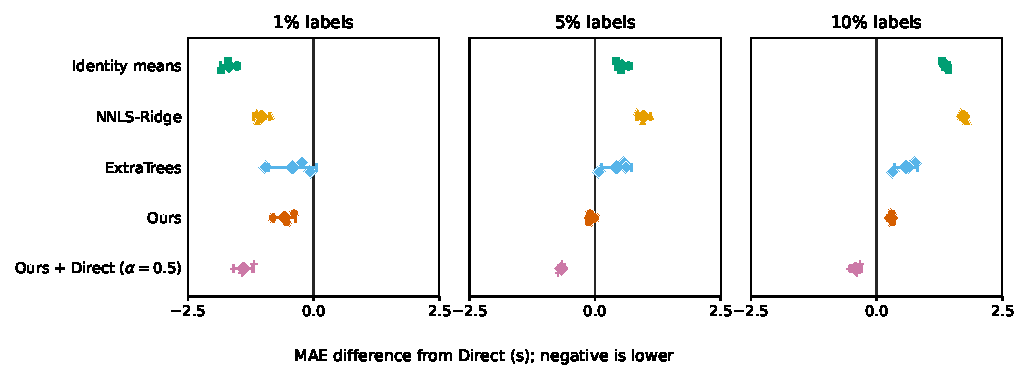
\includegraphics[width=\textwidth]{figures/followup_mae_differences.pdf}
\caption{三个标签布局下相对直接预测的开发集MAE差。负值表示误差较低。神经方法先对每个布局下的三次配对初始化取均值；同段均值和NNLS与对应布局的直接预测均值比较，ExtraTrees与同布局seed 42的直接预测配对。点表示各布局，横线为布局均值及样本标准差。}
\label{fig:comparison}
\end{figure*}

\subsection{标签数量与覆盖范围}
标签预算首先改变可学习信息的数量，但相同数量也可能覆盖不同区间。完整验证标签的布局实验中，将23,720个训练标签限制在每趟前20\%后，可见区间身份从301降为115个，本文方法MAE由28.522增至50.121秒；随机移动40\%连续遮挡保留310个身份，MAE为28.774秒。前缀布局同时改变位置和区间覆盖，原比较无法识别位置的独立作用。该实验完整结果在补充材料中报告。

\begin{table*}[t]
\centering\footnotesize\setlength{\tabcolsep}{4pt}
\caption{同标签总数、身份及每身份标签数量的布局控制：三次初始化、有限验证标签；误差单位为秒。 粗体表示各可比组内的最低误差。}\label{tab:controlled_coverage}
\begin{tabular}{llrr}\toprule
布局 & 方法 & MAE & Prefix50\\\midrule
前20\%标签 & Ours & $\mathbf{50.121\pm0.938}$ & $\mathbf{318.01}$\\
前20\%标签 & 直接预测 & $50.472\pm0.549$ & $326.46$\\
身份计数匹配随机 & Ours & $\mathbf{50.397\pm0.816}$ & $\mathbf{348.30}$\\
身份计数匹配随机 & 直接预测 & $51.374\pm0.609$ & $362.85$\\
\bottomrule\end{tabular}
\end{table*}

为进一步区分这两种变化，采用主实验的有限验证设置，固定前20\%布局并统计115个区间各自的标签数，再从训练数据随机抽取\emph{完全相同的逐区间数量}，总数保持23,720。两种方法共享验证标签、初始化和批次；两种布局的区间集合与计数一致，标签在行程中的位置分布不同。

表\ref{tab:controlled_coverage}中，本文方法在前缀和匹配随机布局下的MAE分别为50.121和50.397秒，直接预测为50.472和51.374秒。随机改变标签位置没有恢复到更广区间覆盖时约29秒的水平，削弱了将全部退化归因于前段位置的解释。该控制只使用一组标签布局，行程和上下文分布尚未完全配平，匹配随机的三次训练均在末步选模。该结果尚不足以确定位置或覆盖的独立贡献。

\subsection{修正机制与消融}
\begin{table*}[t]
\centering\footnotesize\setlength{\tabcolsep}{4pt}
\caption{单独的固定$\rho=0.45$、240步修正控制：三个10\%训练/验证标签布局，每个布局三次配对初始化。误差单位为秒，报告均值与样本标准差。无加权中心化后的缩放也改变有效幅度。粗体表示各可比组内的最低误差。}\label{tab:redistribution}
\begin{tabular}{llrrr}\toprule
变体 & $\rho$ & MAE & RMSE & Prefix50\\\midrule
加权中心化 & 0.10 & $28.849\pm0.189$ & $56.063\pm0.328$ & $145.34$\\
加权中心化 & 0.25 & $28.677\pm0.184$ & $55.503\pm0.353$ & $\mathbf{143.64}$\\
加权中心化（固定$\rho$控制） & 0.45 & $28.633\pm0.239$ & $\mathbf{54.930\pm0.401}$ & $145.26$\\
无加权中心化 & 0.45 & $\mathbf{28.632\pm0.218}$ & $55.030\pm0.227$ & $143.94$\\
\bottomrule\end{tabular}
\end{table*}

修正幅度和加权中心化的比较采用固定$\rho=0.45$的10\%训练/验证设置，每组布局进行三次配对初始化（表\ref{tab:redistribution}）。该控制沿用240步训练协议，与表\ref{tab:limited}中的验证选参、960步主比较分开报告。加权中心化下，$\rho=0.10$、0.25和0.45的MAE分别为28.849、28.677和28.633秒，RMSE分别为56.063、55.503和54.930秒；$\rho=0.25$的Prefix50最低，因此没有一个幅度在所有指标上都占优。

去掉式\eqref{eq:redistribution}中的加权中心化，直接令$r_i=b_i+\rho b_i\tanh z_i$，再执行相同总时长缩放。令$m=\sum_jp_j\tanh z_j$，这一变体的输出可写为
\begin{equation}
\hat t_i^{\mathrm{unc}}=T p_i\left[1+\frac{\rho(\tanh z_i-m)}{1+\rho m}\right].
\end{equation}
相对于式\eqref{eq:shape}，缩放同时改变了有效修正幅度。因此，该比较检验的是两种参数化，不能分离中心化的独立作用。无加权中心化的MAE为28.632秒，与固定$\rho=0.45$中心化控制的28.633秒基本相同。图\ref{fig:ablation}(b)--(d)的配对差值显示指标与运行间存在波动，现有证据没有显示加权零和中心化的精度优势。它保证修正不改变基础时间之和，局部估计是否准确则仍取决于学到的分配。

\begin{table}[t]
\centering\footnotesize\setlength{\tabcolsep}{4pt}
\caption{统一有限训练与验证协议的消融：一组10\%掩码、三次初始化；误差单位为秒。 粗体表示各可比组内的最低误差。}\label{tab:finite_ablation}
\begin{tabular}{lrr}\toprule
变体 & MAE & Prefix50\\\midrule
Ours & $28.709\pm0.396$ & $\mathbf{144.27}$\\
关闭修正 & $29.011\pm0.170$ & $144.66$\\
去日历特征 & $\mathbf{28.588\pm0.132}$ & $148.43$\\
打乱日历特征 & $29.033\pm0.153$ & $151.04$\\
\bottomrule\end{tabular}
\end{table}

表\ref{tab:finite_ablation}汇总三组10\%训练/验证标签布局和每组的三次配对初始化，每个条件共九次观测。关闭行程修正后，MAE由28.633升至29.038秒，九组配对比较均变差。该固定$\rho=0.45$控制表明修正在相同结构内改善了基础估计，但不能证明验证选参后的Ours优于直接预测。

联合打乱日历字段保留了各划分内的字段组合，却破坏其与行程的对应，MAE升至29.010秒，九组配对均高于该固定$\rho=0.45$控制。直接移除日历字段的MAE略低，为28.570秒，但RMSE和Prefix50更高。错配信息与缺少信息的影响不同，现有结果不能证明日历字段不可缺少；两个分支均使用日历上下文，修正收益也不能全部归于某一时间因素。

Singapore辅助实验比较前缀损失的归一化方式。在相同完整标签设置下，包含填充位置、仅计有效位置和不使用前缀目标的本文方法MAE分别为19.518、19.445和19.490秒；仅计有效位置的直接预测为19.545秒。有效位置归一化在三次配对中均略低于对应直接预测和无前缀版本，但长区间误差高于包含填充位置的版本。总体与长区间误差的变化不同；该实验使用完整标签，与Astana稀疏监督条件不同。

\begin{figure}[t]
\centering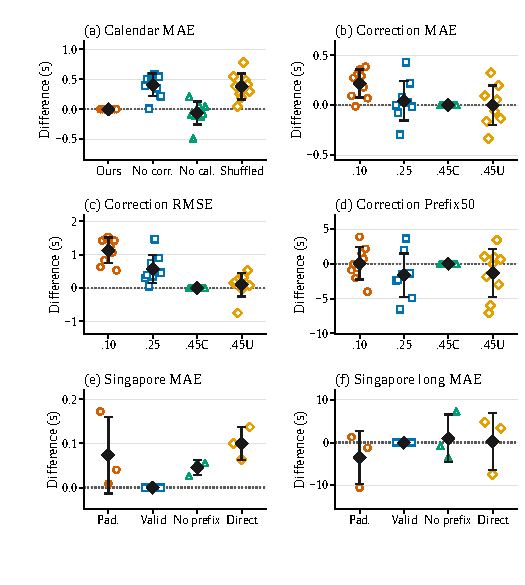
\includegraphics[width=\columnwidth]{figures/ablation_panels.pdf}
\caption{消融的配对误差差值，正值表示误差增加。(a)以Ours为参照，(b)--(d)以加权中心化$\rho=0.45$为参照，(e)--(f)以有效位置前缀目标为参照。空心点为配对运行，实心菱形与误差线为均值和样本标准差；Astana每条件九组，Singapore三组。}
\label{fig:ablation}
\end{figure}

\subsection{逐区间案例与运行效率}
\begin{figure}[t]
\centering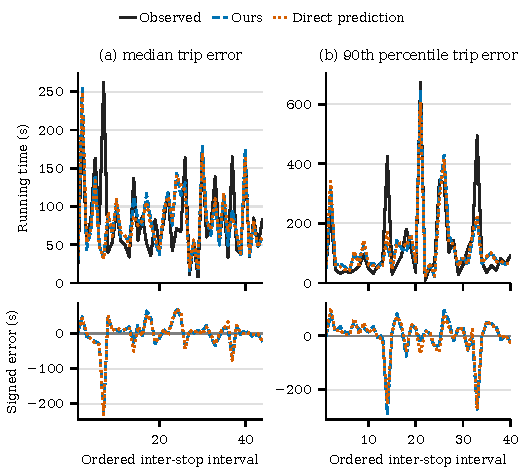
\includegraphics[width=\columnwidth]{figures/local_cases.pdf}
\caption{开发行程的区间时间及有符号误差。从一组10\%标签下的配对运行中，选取Ours行程MAE最接近中位数与90\%分位数的案例。黑、蓝、橙曲线分别表示真实时间、Ours和直接预测。}\label{fig:cases}
\end{figure}
图\ref{fig:cases}展示相同总时长下的局部误差。两例分别含44段和40段，Ours与直接预测MAE分别为25.997/26.486和43.178/43.521秒。部分区间的误差由同一行程中的其他区间补偿，因此总时长一致并不保证局部分配准确。

效率测量使用同一RTX 4090 D、float32和256趟批次，进行10次预热与30次同步计时。两种方法均实例化195,079个参数，实际计算路径不同；前向延迟的中位数与四分位范围见补充材料。计时包含网络前向与总时长缩放，不含数据读取和主机传输。

\subsection{补充评价}
\begin{table*}[t]
\centering\footnotesize\setlength{\tabcolsep}{6pt}
\caption{Singapore完整标签对比：14,933趟OD、295,318个区间。无历史输入方法使用相同给定总时长；strict-past参考额外使用较早行程标签。误差单位为秒；学习型方法报告三次运行的均值与总体标准差。粗体为无历史输入组的最低误差。}
\label{tab:singapore-common-visible}
\begin{tabular}{lrrrr}
\toprule
方法 & 次数 & MAE (s) & RMSE (s) & Prefix50 (s)\\
\midrule
\multicolumn{5}{l}{\textit{common-visible方法}}\\
本文方法（完整标签） & 3 & $\mathbf{19.286\pm0.033}$ & $\mathbf{28.009\pm0.070}$ & $\mathbf{54.938\pm1.043}$\\
MixTTE适配 & 3 & $25.760\pm0.053$ & $35.654\pm0.171$ & $66.292\pm0.255$\\
DutyTTE适配 & 3 & $25.936\pm0.075$ & $35.823\pm0.082$ & $66.805\pm0.515$\\
TriDGNet适配 & 3 & $26.100\pm0.109$ & $36.029\pm0.117$ & $66.782\pm0.502$\\
均匀精确投影 & 1 & $34.399$ & $53.694$ & $102.362$\\
观测弦长精确投影 & 1 & $45.655$ & $60.701$ & $116.574$\\
\midrule
\multicolumn{5}{l}{\textit{历史信息参考方法}}\\
Strict-past direct & 1 & $19.843$ & $36.217$ & $57.385$\\
\bottomrule
\end{tabular}
\end{table*}

表\ref{tab:singapore-common-visible}报告另一个Singapore已知总时长对比，包含14,933个OD和295,318个区间，目标定义与Astana不同。common-visible方法不使用同段历史标签；strict-past参考方法使用此前行程标签，单独列示。Ours沿用相同分配结构，但使用完整局部标签、时长加权和含填充位置的前缀归一化，与Astana稀疏标签协议不同。MixTTE、DutyTTE和TriDGNet为同任务适配\cite{jiang2026mixtte,mao2025dutytte,zuo2026tridgnet}，参数量和训练预算未配平；设置细节见补充材料。结果仅作描述性比较，不构成独立测试。

排除训练及验证中出现过的日期后，2,060趟、82,783段的10\% Ours与直接预测MAE为28.526和28.456秒。未见完整有序路线的子集含446趟、17,164段，两者MAE为35.963和35.315秒。路线组合变化伴随更高误差，但完整路线未见并不等于其中各区间都未见。

补充材料报告七档总时长偏差及训练预算检查。ProbETA适配模型由960延长到3,840步后，MAE从36.403降至32.876秒；一次运行的最优验证点仍在末步，表明其表现受到训练预算影响。

Astana总时长由局部标签求和得到，标签缺失通过人工遮蔽构造。本文报告的是开发集结果，不能估计未触碰测试集上的性能。要评价实际适用性与泛化能力，还需使用独立测量的行程总时长、其他城市数据及完整同任务分解基线。

\section{结论}
本文研究已知总时长下的分段运行时间估计，将同段观测形成的共享估计与当前行程的调整结合起来。基础分支利用区间身份和上下文，行程分支在有界范围内重新分配时间，最后按已知总时长缩放。输出由此保持非负且加和一致，但总时长约束本身不能保证各段准确。

同段均值在标签极少时仍有竞争力。Ours的MAE点估计在1\%和5\%预算下低于直接预测，分别低0.579秒和0.075秒；在10\%下则更高。九组配对运行中，Ours分别在8、6和0组误差较低，且三个预算下的长区间MAE均更高。验证集选出的Ours+Direct集成在5\%和10\%下取得最低平均MAE，但1\%下同段均值仍更低；该集成是独立预测器。现有开发集结果不能证明Ours具有一致优势。相同标签数量在不同区间覆盖下仍产生不同误差。仍需使用独立总时长、未触碰的外部评价集及其他城市数据，判断该分配结构能否改善局部估计。

\bibliographystyle{IEEEtran}
\bibliography{references,additional_references}
\end{document}
